\section{Use of Motion Primitive in Skill Based Framework}
Similar to the concept that speech consist of syllables , it
has been observed that tasks in industrial environments can be broken down into
smaller elements which are called as skills. 
The skills in turn can be decomposed of smaller atomic movements called as Motion Primitives.
A  three layer Framework was introduced by \cite{pedersen_robot_2015} and is illustrated in figure 1.


\begin{figure}[htp]
\centering
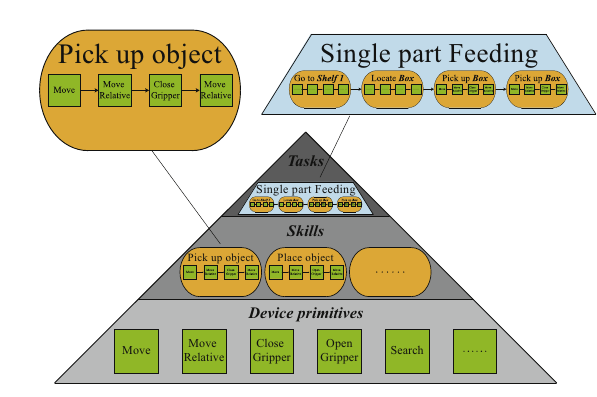
\includegraphics[scale=0.5]{images/skill_framework.png}
\caption[Skill based framework]{Three layers of primitives, skills and tasks. The components in each layer is essentially a combination of lower layer. \cite{pedersen_robot_2015}}
\label{}
\end{figure}

The Three layers can be broken down as follows :
\begin{itemize}
    \item Motion Primitives
    \item Robotics Skills
    \item High Level Tasks
\end{itemize}

\subsection{Motion Primitives}
The lowest layer is the called the motion primitives

% subsection  (end)
\subsection{Robotics Skills}
Robotic skills form the base of the skill based Framework.
Robotic skills are object-centred robot abilities, which can be easily parametrized.
  
% subsection  (end)

\subsection{High level Tasks}
The Higher level description of a task to be done. Ususally in this layer planners like STRIPs or PDDL 
are used to choose which robotic skills has to be executed.

% section  (end)
